\section{補足実験}\label{sec:additional}

\subsection{分類の順位付けとAutoGluonとの照合}

IrisとWineでは、5分類器を学習側の共通分割で比較した。共通の分割を変えて繰り返すと、点順位に加え、反復間の順位の変動を確認できる。順位付けと別に保留した比較用データを用いたWineの例では、他の4候補とCV首位との差の95\%区間がいずれも0を含んだ。これは指定した比較用標本での結果である\cite{ranking,worklog}。

AutoGluon Tabular 1.6.3との比較では、同じ外側のCV分割と最終テストを使った。AutoGluonは各外側foldの学習範囲内で内部検証を行い、外側の評価前に学習範囲全体に再適合した。比較した候補はRandom Forest、Extra Trees、k近傍法、ロジスティック回帰、加重アンサンブルである。LightGBMの試行は実行前の空きメモリ確認で見送った。各ワークフローは候補、前処理、実装が異なるため、同じ分類器の一致試験とは範囲が異なる\cite{agcheck}。

\begin{table}[htbp]
\centering
\small
\caption{同じ最終テスト行でのAutoGluonとDIY AutoMLの照合。差はAutoGluonのmacro F1からDIY AutoMLの値を引いたもの。}
\label{tab:autogluon}
\begin{tabularx}{\linewidth}{@{}p{24mm}YYl@{}}
\toprule
題材 & DIY AutoMLの選定モデルとF1 & AutoGluonの選定モデルとF1 & 差の点推定と95\%区間 \\
\midrule
Iris（30行） & SVM / 0.9666 & k近傍法 / 1.0000 & $+0.0334\ [0.0000,\,0.1023]$ \\
Wine（36行） & SVM / 0.9710 & ロジスティック回帰 / 0.9710 & $0.0000\ [-0.0911,\,0.0911]$ \\
\bottomrule
\end{tabularx}
\end{table}

Irisの差の区間は0に達し、Wineでは0をまたいだ。Wineの混同行列が一致しても、誤分類した行は二つの方法で異なった。選定後の予測に条件付けた区間と、小規模な開発用データの範囲で読む必要がある。

\subsection{深層学習バックエンドと予測確率}

WindowsのCPU上でTensorFlow CPU 2.20.0、Keras 3.15.1とPyTorch 2.14.0を比較した。IrisとWineに対し、同じ分割、標準化、MLPの構成（隠れ層32、16、8）、初期重み、ミニバッチ順を用い、学習seed 42、43、44でそれぞれ学習した。共通重みの推論と、両バックエンドで独立に学習した後の予測を分けて照合した\cite{dlcheck}。

共通重みでの最大確率差は概ね \(6\times10^{-8}\) だった。学習後のテスト行・クラス・seed全体での最大絶対確率差は、Irisで0.03053、Wineで0.00211だった。両データの分類ラベルは各seedで行ごとに一致し、macro F1も一致した。予測確率を費用や閾値の計算に使う場合は、ハードラベルで確認できた一致に加え、確率の差と校正を調べる余地がある。

保存済みlogitから計算した3 seed平均のlog loss差（PyTorchからTensorFlowを引く）はIrisで \(-0.002212\)、Wineで \(-0.00006439\) だった。Irisの1,000回の行再標本化による95\%区間は \([-0.005877,\,0.000602]\) だった。Wineでは同じ乱数列を1,000回から20,000回に延ばすと、区間の上端が \(-3.0\times10^{-7}\) から \(+1.8\times10^{-7}\) に変わった。反復数の変更は、同一予測に条件付けた区間の数値的な変動を確認する操作である。独立な学習データや追加のseedによる新しい検証は別途必要になる\cite{dlprob}。

\subsection{数値計算と仮の校正ずれ}

順位付けの検証では、保持した分類器のテスト入力をFloat32へ丸めてから戻し、IrisとWineの予測ラベルに変化がないことを確認した。Irisでテストの花弁幅すべてに \(+0.5\) cmを加える仮定では、30件中6件で予測が変わり、macro F1は0.9666から0.7341へ変わった。前者は指定した丸め、後者は一定の入力オフセットに対する感度である。実際の測定の偏り、推論器の全演算を低精度にした場合、分布の変化は、条件を変えた別の検証で扱う\cite{ranking,worklog}。

\subsection{Annealing checkによる任意の特徴量探索}

Annealing checkは、分類器を固定して特徴量の部分集合を選ぶCPUの任意実行である。焼きなまし法\cite{kirkpatrick}の近傍は1列の追加・削除、または1列の交換で作る。探索に使う指標は共通の学習側CVでのmacro F1である。比較には同じ候補評価数のランダム探索と全列モデルを置き、小さい探索空間では全列挙も照合に使う。候補、温度、受理の経過と実際の学習回数を保存する\cite{annealing}。

Irisでは4特徴量の非空15候補を全列挙し、全列のCV F1 0.9707が最高だった。各手法8候補の予算で、10探索seedのうち焼きなまし法は3回、ランダム探索は8回、このCV最良値に達した。Wineでは13特徴量から最大6列を選び、手法ごとに32候補、320回のCV学習を割り当てた。CVでは各手法が10探索seedのうち5回ずつ上回った。IrisとWineの各seedで、保留macro F1の焼きなまし法とランダム探索の差に付けた95\%区間は0を含んだ。共通の保留標本で探索seedを変えた結果なので、10回を独立な外部検証として数えない。量子アニーリングとQUBOは別の研究課題に残す。

\subsection{16\,GBのWindows端末での点検と学習}

Windows、Intel Core i5-14400、物理メモリ約16\,GB、Python 3.13.17の端末で、模擬数値CSVの点検、作業用Parquetへの変換、選択行の抽出、抽出後のモデル比較を個別に測った。固定seedで整数特徴量を作り、一部の加重和から二値ラベルを作った。各工程を3回実行し、時間はCLI起動から終了までの中央値とした。BLASとOpenMPは1スレッドとし、ピークメモリはCLIプロセスのワーキングセットで測った\cite{scalebench}。

\begin{figure}[htbp]
\centering
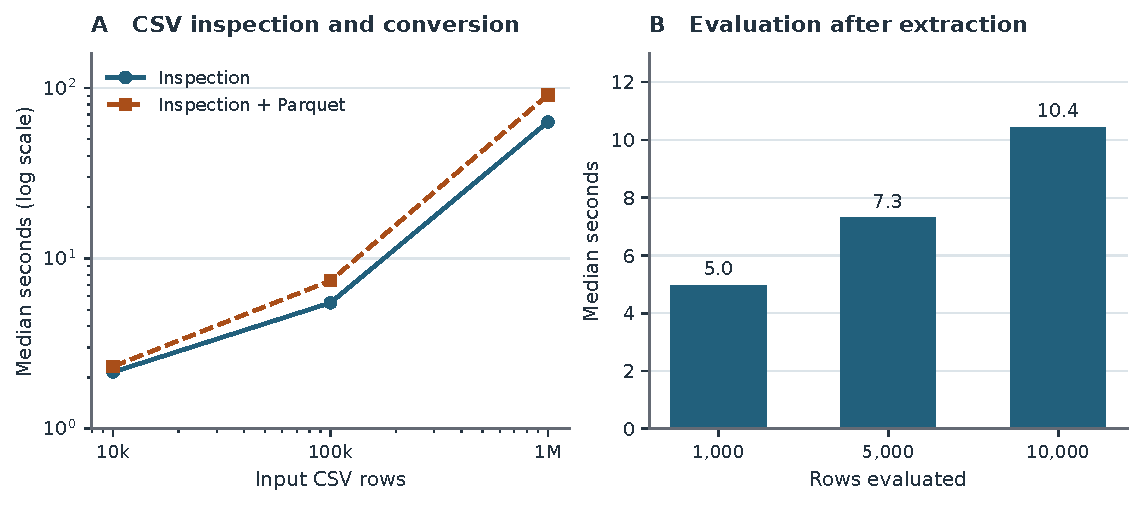
\includegraphics[width=\linewidth]{processing_cost.pdf}
\caption{模擬データの処理時間。左は7特徴量のCSV点検と作業用Parquetへの変換で、両軸を対数表示。右は7特徴量の抽出済みCSVに対する5モデルの比較・保留評価・保存の所要時間。各値は工程ごとに3回測った中央値。}
\label{fig:scale}
\end{figure}

100万行・7特徴量のCSVは36.2\,MB、作業用Parquetは18.9\,MBだった。点検だけは63.3秒、点検と変換は91.1秒を要した。作成済みParquetから2条件を満たす先頭1万行を抽出する工程は2.3秒で、5モデルの比較と保留テストを含む評価工程は10.4秒だった。5,000行では7特徴量の評価が7.3秒、28特徴量が11.6秒だった。100万行は点検・保存の規模であり、学習を計測した最大規模は1万行である。図\ref{fig:scale}はこの端末と数値データの結果で、データ型、列数、ファイルキャッシュ、実行するモデルが変われば負荷も変わる。
